\documentclass[11pt]{article}
\usepackage{amsmath}
\usepackage{siunitx}
\usepackage{tikz}
\usepackage{graphicx}
\usepackage{longtable}
\usepackage{multirow}
\usepackage{adjustbox}
\usepackage{pifont}
\usepackage{ulem}
\usepackage{xcolor,colortbl}
\usepackage{pgfplots}
\usepackage{float}
\usepackage{amsmath}
\usepackage{listings}
\usepackage{hyperref}
\usepackage{graphicx}
\usepackage{subcaption}
\hypersetup{
    colorlinks=true,
    linkcolor=blue,
    filecolor=magenta,      
    urlcolor=cyan,
}
\usepackage{amsmath}
\usepackage{xepersian}
\settextfont{XB Niloofar}
\setlatintextfont{Linux Libertine O}
\setdigitfont{XB Niloofar}
\title{پاسخ سوالات تیوری پروژه‌ی مبانی بیو‌انفورماتیک}
\author{میلاد آقاجوهری ، احسان سلطان‌آقایی}
\begin{document}
\maketitle
\section{سوال اول}
\subsection{سوال اول بخش دوم یا اولین سوال تیوری}
شناخت ژنوم ویروس ابولا:


۱. گلیکوپروتیین وظیفه متصل شدن به گیرنده های روی سطح سلول برای هدایت ژنوم ابولا به درون سلول را  دارد و با زنجیره کربوهیدراتی پوشید ه شده است که آن را از سیستم ایمنی مخفی نگه می دارد. گلیکوپروتیین از سطح ویروس گسترش می یابد و ویروس و سلول را به اندازه  کافی به هم نزدیک می کند تا غشاها به یک دیگر متصل شوند. GP  تنها پروتیئن بیان شده توسط ابولا است که در غشای سطح سلول است.
عوامل متعددی برای ویروس ابولا مورد نیاز است تا بتواند به سلول میزبان دسترسی پیدا کند. یکی از اجزای مورد نیاز برای ورود به سلول میزبان گلیکوپروتیئن ها هستند که فیلوویروس ها را به سطح میزبان متصل می کنند، ویروس ها را به اندوسوم ها می فرستند و به همجوشی بین ویروس وغشای اندوسوم کمک می کنند.
به عبارتی این پروتئین مسئول متصل شدن ویروس وآلوده کردن سلول میزبان است و هم چنین درمختل کردن چسبندگی سلول ها موثر است. فلذا می تواند پروتئین منجر به بیماری قلمداد شود ولی یکی دیگر از پروتئین ها VP24  نیز می تواند مقصود باشد که در ادامه آن را ذکر خواهیم کرد.

۲. پروتیین ماتریس ابولا ( Ebola Matrix Protein ) که با نام VP40 شناخته می شود و در فرآیند جوانه زنی موثر است. (نقش این فرآیند دربخش بعدی سوال توضیح داده خواهد شد)
 نمونه های زیادی از این پروتیین مربوط به غشا است و به نظر می رسد که با هر دوغشا و نوکلئوکپسید در ارتباط است. 
هم چنین از آن جایی که ویروس ها درون ژنومشان تنها  فضا برای کدگذاری تعداد کمی پروتیین دارند اکثر پروتیین ها چندین وظیفه برعهده دارند. برای مثال پروتیین ماتریس در ابولا ساختار های کاملا متفاوتی برای وظایف مختلفش به خود میگیرد: به عنوان هگزامر درساختار ویریون ( فرم ویروس در خارج از سلول میزبان) شرکت دارد،  به عنوان اکتامر به RNA متصل می شود و رونویسی آن را تنظیم می کند و به عنوان دیامر در حمل پروتیین موثر است.


در مرکز ویروس مجموعه پروتیین های نوکلئوکپسید از ژنوم محافظت می کنند که با نام های  VP24 , VP30 , VP35 , NP  شناخته می شوند. اطلاعات ژنتیکی ویروس ابولا در نوکلئوکپسید است. زمانی که ابولا با موفقیت وارد سلول میزبان شد ترجمه و رونویسی آن را می رباید.

۳. ویروس ابولا  تب همراه با  مرگ و میر به احتمال ۹۰ درصد را ایجاد می کند و در موارد مرگ و میر،  ناشی از سرکوب اولیه سیستم ایمنی ذاتی میزبان است. یکی از پروتئین هایی که ادر این مورد تاثیر می گذارد VP24 است که سیگنال اینترفرون را متوقف می کند. در نتیجه به عبارتی می‌توان این پروتئین را که سیستم ایمنی را مختل می‌کند باعث ایجاد بیماری دانست.

۴. رونویسی ویروس ابولا وابسته به VP30 است و یک Transcription Factor از نوع Activator برای ویروس ابولا است و به وسیله تثبیت mRNA به رونویسی ویروس کمک می کند.

۵. پروتئین VP35 همانطور که در بالا گفته شد چند منظوره است و به عنوان یکی از اجزای مجموعه RNA پلیمراز، عامل مونتاژ ویروس و مهارکننده تولید اینترفرون میزبان عمل می کند.

۶. نوکلئوپروتیین(NP)  دور RNA می پیچید و یک مجموعه مارپیچی تشکیل می دهد. این پروتئین فراوان ترین پروتئین در سلول آلوده و در مجموعه نوکلئوکپسید است. هم چنین  به شدت با ژنوم ویروس در ارتباط است و در رونویسی ویروس (Transcription) ،  تکثیر RNA ، بسته بندی ژنوم و سر هم کردن نوکلئوکپسید قبل از کپسوله سازی غشا مورد نیاز و موثر است.

۷. پروتیین L  که یک RNA پلیمراز وابسته به RNA است و بسیاری از نمونه های جدید ژنوم RNA را می سازد. (RNA Replication)

پروتئین های ماتریس و VP24 و VP30 و VP35 و نوکلئوپروتئین وL  پروتئین های ساختاری هستند و خود پروتئین GP نیز ساختاری است ولی پروتئین های sGP , ssGP , delta غیرساختاری هستند که حاصل ویرایش و پردازش پس از ترجمه ژن GP  و محصولات ژن هستند. SGP می تواند نقش مهمی در فرار از پاسخ ایمنی هومورال با جذب آنتی بادی های ایجاد شده داشته باشد.


\subsection{سوال اول بخش سوم}

 نحوه وارد شدن ویروس ابولا به درون سلول و آلوده کردن آن:

ویروس ابولا از ماکروپینوسیتوز(macropinocytosis)  به منظور دسترسی به سلول های میزبان هدف خود و انتقال خود به داخل سلول استفاده می کند.ماکروپینوسیتوز فرآیندی است که در آن بخش های رفع غشای پلاسما خارج از سلول به صورت به خود برگشته ای قرار میگیرند که حفره هایی ایجاد می شود (ماکروپینوزوم)  و ویروس به کمک گلیکوپروتئین به سطح غشای پلاسما متصل می شود. شکل گیری ماکروپینوزوم به صورت خود به خودی به علت فعال شدن عوامل مختلف رشد یا به طور همزمان با مصرف مولکول های سلولی یا مایع خارج سلولی اتفاق می افتد. سپس غشا روی ویروس بسته می شود و ویروس همراه با مولکول های دیگر و مایعات خارج سلولی، تشکیل یک کیسه کوچک می‌دهند و به درون سلول منتقل می‌شوند.

NPC1  پروتئین حمل کننده کلسترول اندوسوم و لیزوزوم است که درغشای لیزوزوم یافت می‌شود و برای آلوده کردن سلول میزبان مورد نیاز است. ( درصورت فقدان این پروتئین ویروس نمی‌تواند سلول را آلوده کند ولی خود سلول نیزنمی تواند در فقدان این پروتئین  به حیات خود ادامه دهد)
هنگامی که ویروسی درون سلول قرار دارد، NPC1  به همجوشی فیبر ویروس با اندوسوم و لیزوزوم کمک می کند و پس از آن ویروس می تواند کیسه (vesicle) خود را ترک کند وتکثیر شود.(علاوه بر NPC1  مجتمع HOPS نیز به عنوان عامل مهمی در روند عفونت ویروسی شناخته شده است.)

پس از ترک کیسه ویروس دستگاه رونویسی سلول را می‌رباید تا بتواند خود را تکثیر کند و در این صورت دیگر سلول نمی‌تواند اجزای مورد نیاز خود را از طریق رونویسی به دست آورد و منجر به مرگ سلول و یا ناتوانی آن در عملکرد مناسب می‌شود. زمانی که تمام اجزای مورد نیاز برای تشکیل یک ویروس جدید فراهم شدند اجزای ویروس از سلول جوانه می‌زنند و به وسیله غشای سلول برای خود کپسول درست می‌کنند تا بتوانند سفر امنی به سلول مجاور داشته باشند و عملیات آلوده کردن سلول‌ها را ادمه دهند.


نحوه آلوده و عفونی کردن بدن و از بین بردن میزبان:

ویروس ابولا پس از وارد شدن به بدن سلول‌های خاصی را مورد هدف قرار می‌دهد از جمله سلول‌های کبدی، سلول‌های سیستم ایمنی بدن و سلول‌های اندوتلیال که داخل رگ‌های خونی قرار دارد. ابولا انواع سلول ها را می تواند آلوده کند واین قابلیت آن را یک عامل عفونی بسیار موفق می کند.

 ویروس ابولا درون سلول به کمک گلیکوپروتئین چسبندگی سلول را مختل می‌کند و در نتیجه سلول‌ها در چسبیدن به هم و تشکیل ماتریس خارج سلولی (که در بافت های سالم کمک به کنار هم نگه داشته شدن سلول‌ها کنار یک دیگر می‌شود) دچار مشکل می‌شوند. از دست دادن چسبندگی سلول برای هر بافت جامدی زیان آور است.
ویروس ابولا با آلوده کردن  سلول‌های رگ‌های خونی  باعث ایجاد سوراخ  در آن و خونریزی داخلی می‌شود. هم چنین با هدف قرار دادن سلول های کبدی، توانایی بدن برای پاک کردن سموم از جریان خون به خطرمی افتد  و با آلوده سازی سیستم ایمنی بدن که سلول های آن در همه جا در بدن حرکت می کنند، ابولا می تواند به سرعت در حال افزایش سطح عفونت خود باشد. با گذشت زمان، عفونت سلول ها در سراسر بدن می تواند باعث نارسایی اندام شود و تب، خونریزی داخلی، اسهال و استفراغ می تواند باعث کاهش شدید الکترولیت ها، پلاسمای خون و مایع شود و در نهایت، نارسایی اندام و شوک ناشی از خونریزی داخلی منجر به مرگ می‌شود.
و رفرنس‌ها:

\href{http://pdb101.rcsb.org/motm/178}{[1]}
\href{https://microbewiki.kenyon.edu/index.php/Ebola_virus_entry_into_host_cells}{[2]}
\href{http://sitn.hms.harvard.edu/flash/2014/ebola-virus-how-it-infects-people-and-how-scientists-are-working-to-cure-it/}{[3]}
\href{https://www.omicsonline.org/open-access/ebola-virus-disease-a-biological-and-epidemiological-perspective-of-avirulent-virus-jidd-1000103.php?aid=71427&view=mobile}{[4]}
\href{https://en.wikipedia.org/wiki/Ebola_virus_disease}{[5]}
\href{https://www.ncbi.nlm.nih.gov/pmc/articles/PMC2829775/}{[6]}
\href{https://www.rcsb.org/structure/4qb0}{[7]}
\href{https://www.rcsb.org/structure/3vne}{[8]}
\href{https://www.rcsb.org/structure/3fke}{[9]}
\href{https://www.rcsb.org/structure/2i8b}{[10]} 
\subsection{تشکیل درخت زندگی برای هر ژن}
\subsubsection{مقایسه‌ی نتایج الگوریتم برای ۵ ژن}
در ابتدا تمامی نتایج حاصله را روبروی هم مشاهده می‌کنیم:
\begin{figure}[h]
  \centering
  \begin{subfigure}[b]{0.4\linewidth}
    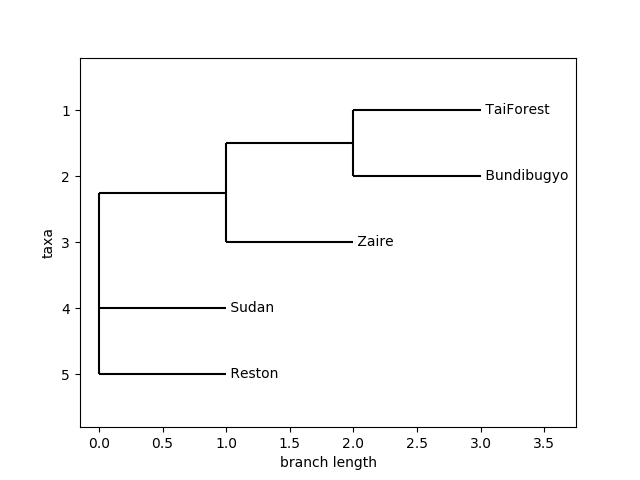
\includegraphics[width=\linewidth]{../Data/Trees/NP_NJ.png}
    \caption{NP\_NJ.png}
  \end{subfigure}
  \begin{subfigure}[b]{0.4\linewidth}
    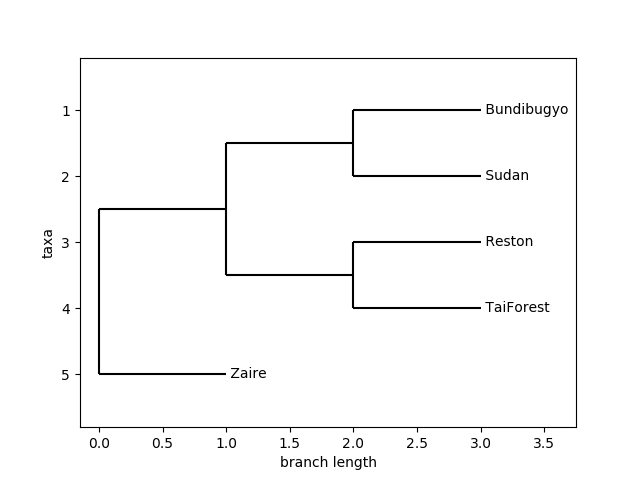
\includegraphics[width=\linewidth]{../Data/Trees/NP_UPGMA.png}
    \caption{NP\_UPGMA.png}
  \end{subfigure}
\end{figure}
\newline
برای این ژن درخت‌های حاصل یکی هستند.
\newline
\begin{figure}[H]
  \centering
  \begin{subfigure}[b]{0.4\linewidth}
    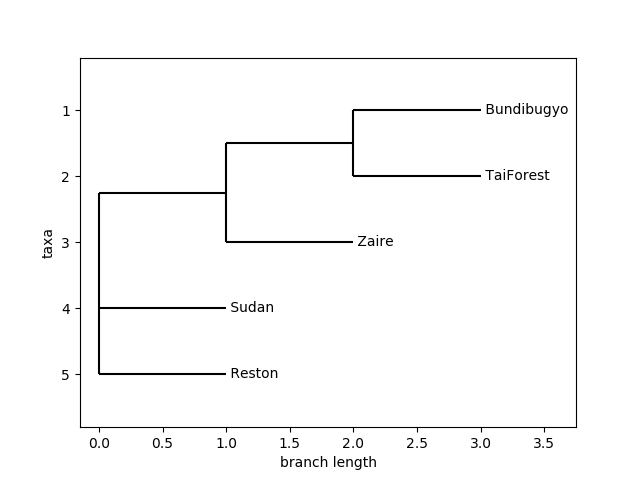
\includegraphics[width=\linewidth]{../Data/Trees/VP35_NJ.png}
    \caption{Vp35\_NJ.png}
  \end{subfigure}
  \begin{subfigure}[b]{0.4\linewidth}
    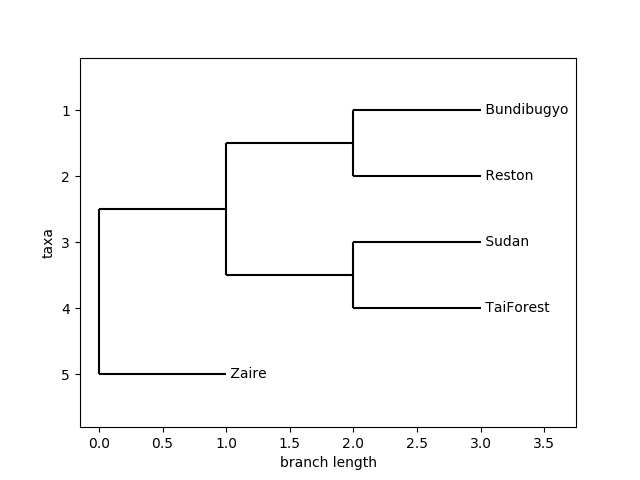
\includegraphics[width=\linewidth]{../Data/Trees/VP35_UPGMA.png}
    \caption{VP35\_UPGMA.png}
  \end{subfigure}
\end{figure}
برای این ژن درخت‌های حاصل یکی هستند(در واقع یک مفهوم را میرسانند).
\newline
\begin{figure}[H]
  \centering
  \begin{subfigure}[b]{0.4\linewidth}
    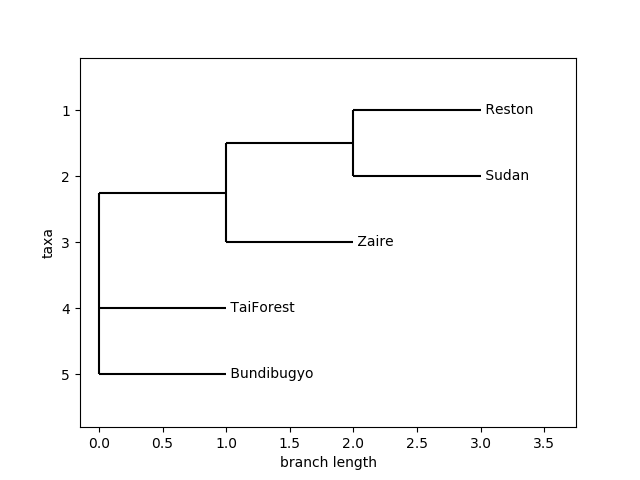
\includegraphics[width=\linewidth]{../Data/Trees/VP40_NJ.png}
    \caption{Vp40\_NJ.png}
  \end{subfigure}
  \begin{subfigure}[b]{0.4\linewidth}
    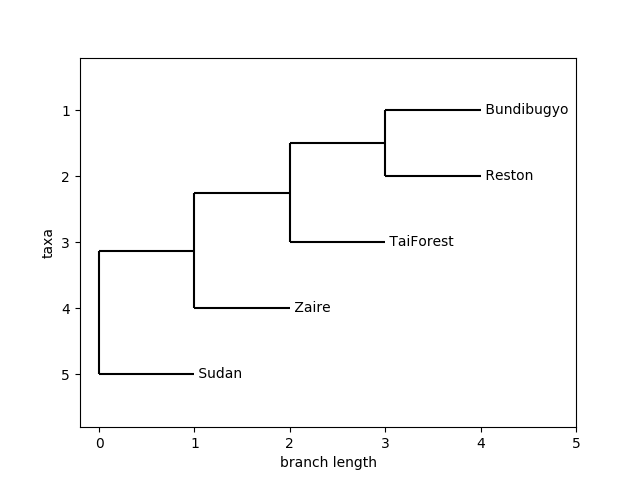
\includegraphics[width=\linewidth]{../Data/Trees/VP40_UPGMA.png}
    \caption{VP40\_UPGMA.png}
  \end{subfigure}
\end{figure}
برای این ژن درخت‌های حاصل تفاوت جزیی دارند، البته معنایشان تقریبا یکسان است، صرفا UPGMA اطلاعات بیشتری داده است.
\newline
\begin{figure}[H]
  \centering
  \begin{subfigure}[b]{0.4\linewidth}
    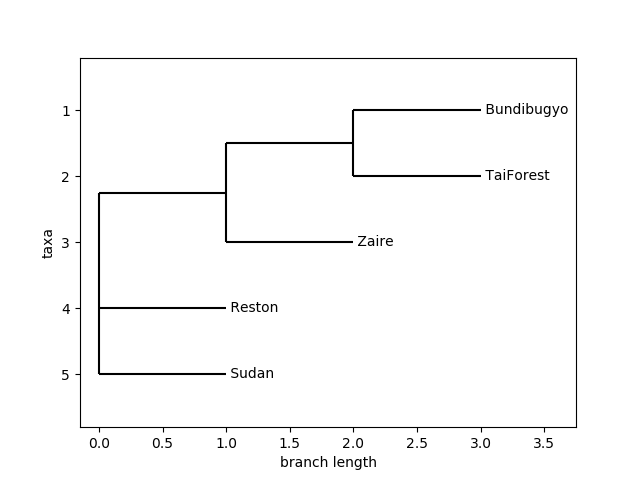
\includegraphics[width=\linewidth]{../Data/Trees/GP_NJ.png}
    \caption{GP\_NJ.png}
  \end{subfigure}
  \begin{subfigure}[b]{0.4\linewidth}
    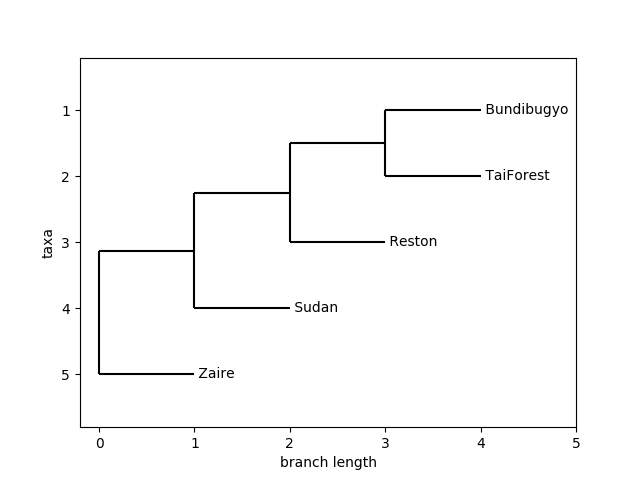
\includegraphics[width=\linewidth]{../Data/Trees/GP_UPGMA.png}
    \caption{GP\_UPGMA.png}
  \end{subfigure}
\end{figure}
درخت‌های حاصل در این جا بسیار متفاوت هستند و تنها در مورد Bundibugyoو TaiForest یکسان هستند.
\begin{figure}[H]
  \centering
  \begin{subfigure}[b]{0.4\linewidth}
    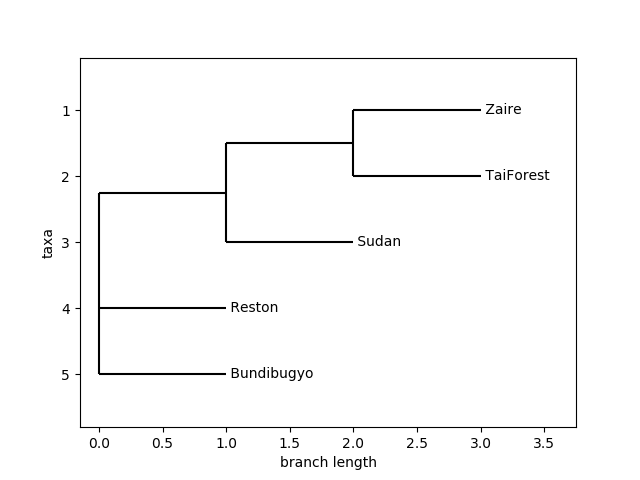
\includegraphics[width=\linewidth]{../Data/Trees/VP30_NJ.png}
    \caption{VP30\_NJ.png}
  \end{subfigure}
  \begin{subfigure}[b]{0.4\linewidth}
    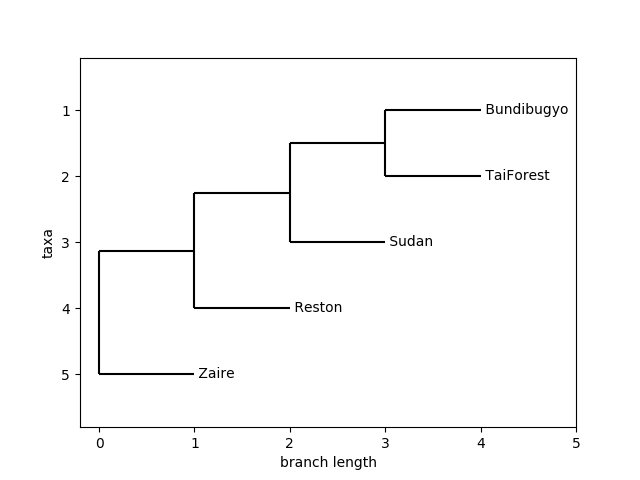
\includegraphics[width=\linewidth]{../Data/Trees/VP30_UPGMA.png}
    \caption{VP30\_UPGMA.png}
  \end{subfigure}
\end{figure}
در این‌جا درخت‌های حاصل تفاوت زیادی دارند.
\begin{figure}[H]
  \centering
  \begin{subfigure}[b]{0.4\linewidth}
    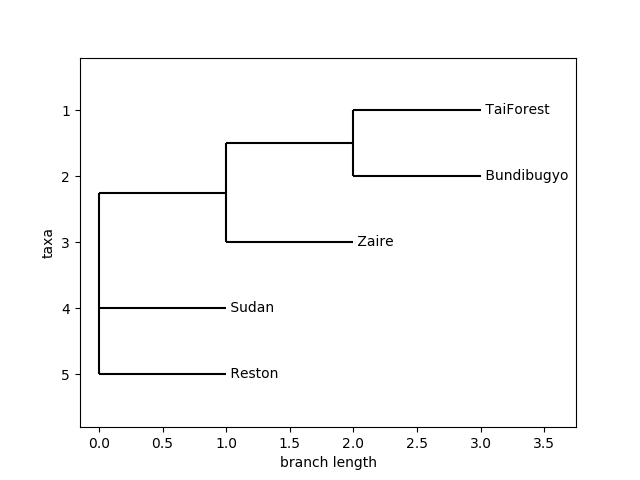
\includegraphics[width=\linewidth]{../Data/Trees/VP24_NJ.png}
    \caption{VP24\_NJ.png}
  \end{subfigure}
  \begin{subfigure}[b]{0.4\linewidth}
    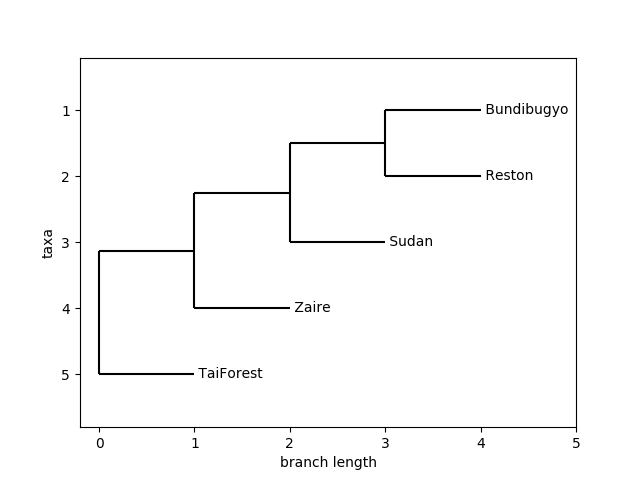
\includegraphics[width=\linewidth]{../Data/Trees/VP24_UPGMA.png}
    \caption{VP24\_UPGMA.png}
  \end{subfigure}
\end{figure}
تنها در قسمت Zaire و Bundibugyo تفاوت در درخت‌‌ها هست.
\begin{figure}[H]
  \centering
  \begin{subfigure}[b]{0.4\linewidth}
    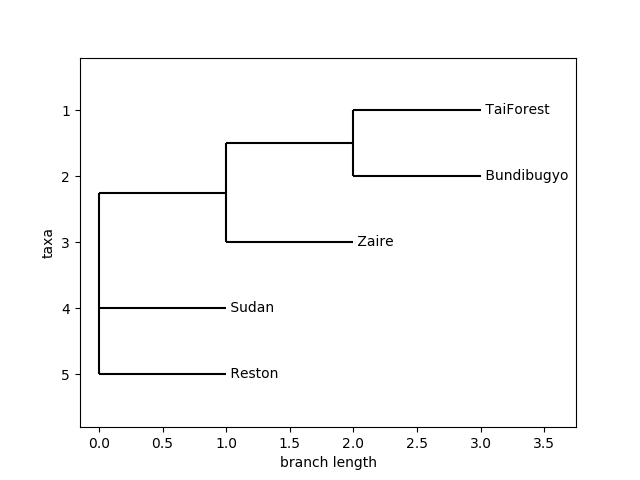
\includegraphics[width=\linewidth]{../Data/Trees/L_NJ.png}
    \caption{L\_NJ.png}
  \end{subfigure}
  \begin{subfigure}[b]{0.4\linewidth}
    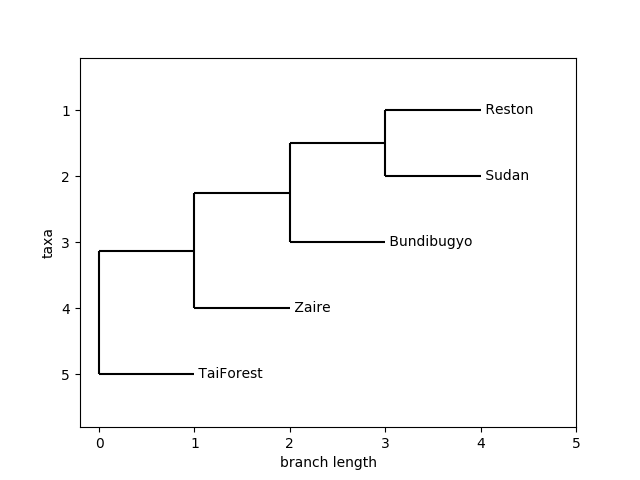
\includegraphics[width=\linewidth]{../Data/Trees/L_UPGMA.png}
    \caption{L\_UPGMA.png}
  \end{subfigure}
\end{figure}
در اینجا هر دو درخت یک مفهوم را میرسانند اگرچه ظاهرا تفاوت جزیی مشاهده می‌شود.
\newpage
\subsection{مقایسه‌ی نتایج}
نمی‌توان گفت نتایج تفاوت‌ها‌ي چشم‌گیر دارند. مخصوصا اینکه در NJ در چهار ژن به یک درخت رسیده‌ایم که در سه عدد از UPGMA ‌ها هم همین درخت حاصل شده‌است اما به هر حال نتایج در مورد بعضی‌ ‌ژن‌ها تفاوت دارند.
\subsubsection{بیان دلیل تفاوت‌ها}
بستگی دارد منظور کدام نوع از تفاوت‌ها باشد. اگر منظور تفاوت‌های بین نتایج دو الگوریتم است، که این دو الگوریتم فرض‌های متفاوتی در مورد درخت اصلی دارند که به آن‌ها در قسمت‌های قبلی اشاره شده و منطقی است که نتایج متفاوت باشد. مثلا UPGMA تاکید دارد که فاصله‌ي تمام برگ‌ها از درخت ریشه یکسان باشد.

اگر منظور تفاوت‌‌های بین درخت‌های حاصل برای ژن‌هاست، الزاما جهش‌های ژنی روند درختی دقیق ایجاد ویروس‌های جدید را دنبال نمی‌کنند، مثلا ممکن است یک نوع از ویروس در یک جایگاه مثلا جایگاه پنجاهم که در ژن سوم است جهش کند اما انواع دیگر نکنند، در این‌جا روش‌های ما این ویروس را جدا از بقیه ترسیم می‌کند و حتی او را از تمام برادران و پدرانش در یک دسته‌ی جدا میگذارد. پس الزاما بر حسب یک ژن نمی‌توان تصمیم گرفت که روند جهش ها و تولید گونه های جدید ویروس چه بوده است اما با ترکیب آن‌ها می‌توان دقت بیشتری در این امر به دست آورد.
\subsubsection{مقایسه‌ی دو الگوریتم NJ , UPGMA}
مزیت بزرگ الگوریتم UPGMA، محاسبه‌ی درخت‌های ریشه‌دار است. این الگوریتم با فرض یکسان بودن فاصله‌ی تمام برگ‌ها از ریشه درخت را محاسبه می‌کند، این فرضی است که در بسیاری از موارد نادرست است. فرض دیگر این الگوریتم ثابت بودن نرخ تکامل است(که من متوجه نمی‌شوم این فرض در کجای این الگوریتم هست  ناشی از عدم تسلط من به ریاضی پشت منطق این الگوریتم است). ثابت فرض کردن نرخ تکامل را نمی‌توان یک نقطه‌ی ضعف در نظر گرفت، زیرا طبق مطالبی که در ویکیپدیا خواندم اکثر کاربرد‌های این الگوریتم در مواقعی است که می‌خواهند بدون در نظر گرفتن نرخ تکاملی بین توالی‌ها و تنها با دقت به شباهت‌ آن‌ها، آن‌ها را گروه‌بندی کند که در شاخه‌ای به نام Phenetics که هدف آن دسته‌بندی میان موجودات بر حسب مشاهدات کلی است، روشی مناسب است.

به نظر من حتی در همین پروژه دیدیم که این الگوریتم در زمینه‌ی دسته‌بندی بر حسب ژن‌ها چندان هم خوب عمل نکرد و درخت‌های نسبتا متفاوتی را برای هر ژن نتیجه می‌داد  البته اجماع تمام آن‌ها به درختی صحیح منتهی شد که  نتیجه منطبق با نتیجه‌ي ترکیب‌شده‌ی NJ بود و البته طبق بررسی‌های
 \textit{
 یواشکی :)
 }
 ما در اینترنت با نتیجه‌ي درست هم منطبق است. 

نکته‌ی منفی الگوریتم NJ تولید درخت‌های بدون ریشه است، اما نکته‌ي مثبت آن عدم فرض یکسان بودن نرخ تکامل است(البته من متوجه نمی‌شوم که این فرض در کجای الگوریتم هست که ناشی از عدم تسلط من به ریاضی پشت منطق این الگوریتم است).همین فرض مثبت این الگوریتم ٔآن را برای بررسی داده‌‌های توالی بسیار مناسب کرده است. نقطه‌ی مثبت دیگر این الگوریتم سریع بودن آن در قیاس با روش‌های دیگر است که آن را برای بررسی داده‌های در مقیاس بزرگ و استفاده از روش‌های آماری که بارها از داده نمونه‌برداری می‌کنند(مانند bootstrap) مناسب کرده‌است. این روش در صورتی که ماتریس فاصله‌ها درست باشد، پاسخ صحیح را تولید می‌کند، اما حتی اگر ماتریس فاصله‌ها درست نباشد و حدودا درست باشد، این الگوریتم به طرز معجزه‌آسایی به احتمال خوبی باز هم درخت درست را تولید می‌کند(شهودی در مورد این که این اتفاق چرا می‌افتد پیدا نکردم، حتی ویکیپدیای انگلیسی از لفظ
\lr{but neighbor joining often constructs the correct tree topology anyway}
) استفاده کرده‌‌است و به یک مقاله‌
\href{https://arxiv.org/abs/cs/0602041}{(اینجا)}
 لینک داده است که فرصت نشد مطالعه کنم.  این الگوریتم به بعضی از شاخه‌ها وزن منفی می‌دهد و این نامطلوب است(این در ویکیپدیا گفته شده، اما ما در این تمرین مشاهده نکردیم).
 \subsection{ترکیب درخت‌ها و ارائه‌ی درخت نهایی}
 ما در اینجا از پکیج
 \lr{ape}
 متد
 \lr{consensus}
 استفاده کردیم. در این روش ما از احتمال برابر با 0.5 استفاده کردیم به این صورت است که یا‌ل‌‌هایی را که در ۵۰ درصد یا بیش‌تر از درخت‌ها آمده است با همدیگر ترکیب می‌‌کند و یک 
 \lr{majority rule consensus tree}
 حاصل می‌کند. این روش روش مناسبی به نظر می‌رسد چرا که به هر یال به اندازه‌ای که تکرار شده وزن و اهمیت می‌دهد و در واقع روش مبتنی بر اهمیت دادن به یال‌های آمده در روش‌هاست.(البته واژه‌ی یال در این‌جا بار معنایی مناسب و دقیق را ندارد و منظور ما در اینجا از یال 
 \lr{clade}
 است.
  )گویا این الگوریتم یال‌ها را بر حسب تعداد تکرار مرتب می‌کند و سعی می‌کند درختی تولید کند که با اکثر آن‌ها که بالای ۵۰ هستند بخواند.
 \subsection{مقایسه‌ی درخت ترکیبی و درخت حاصل از همترازی سراسری}
 ابتدا درخت حاصل از همترازی سراسری را مشاهده می‌کنیم.
\begin{figure}[H]
  \centering
  \begin{subfigure}[b]{0.4\linewidth}
    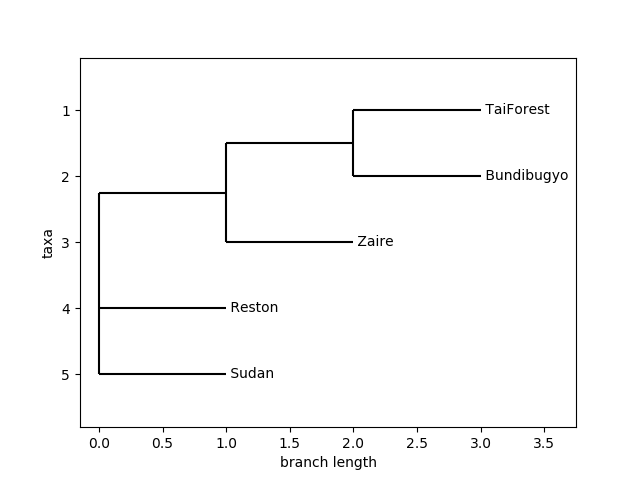
\includegraphics[width=\linewidth]{../Data/Trees/genome_NJ.png}
    \caption{genome\_NJ.png}
  \end{subfigure}
  \begin{subfigure}[b]{0.4\linewidth}
    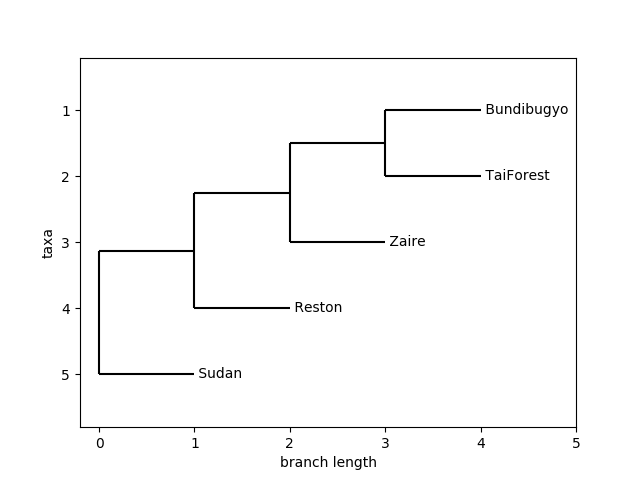
\includegraphics[width=\linewidth]{../Data/Trees/genome_UPGMA.png}
    \caption{genome\_UPGMA.png}
  \end{subfigure}
\end{figure}
و سپس درخت‌های ترکیبی را مشاهده می‌کنیم:
\begin{figure}[H]
  \centering
  \begin{subfigure}[b]{0.4\linewidth}
    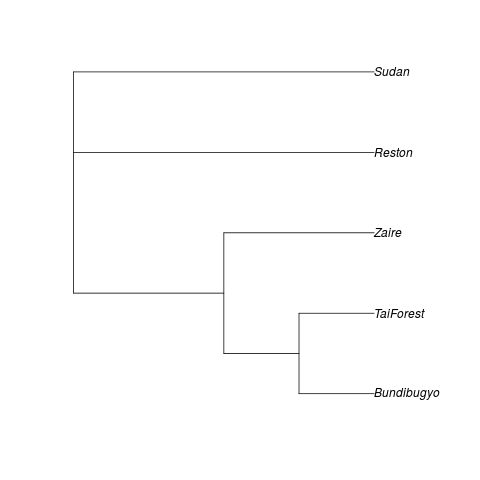
\includegraphics[width=\linewidth]{../Data/Trees/NJ.png}
    \caption{mix\_NJ.png}
  \end{subfigure}
  \begin{subfigure}[b]{0.4\linewidth}
    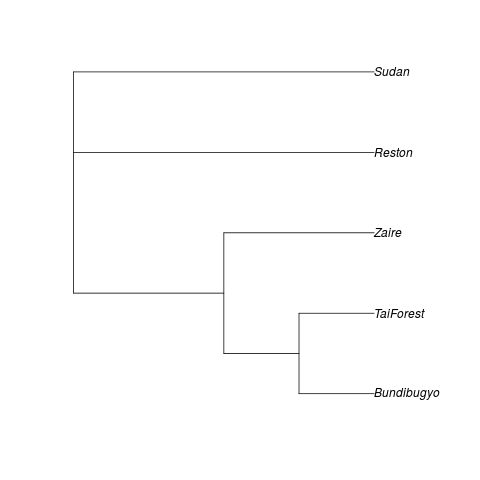
\includegraphics[width=\linewidth]{../Data/Trees/UPGMA.png}
    \caption{mix\_UPGMA.png}
  \end{subfigure}
\end{figure}

همانطور که مشاهده می‌شود تمام این نتایج یکسان هستند و چندان مقایسه‌ای نداریم:).
\subsection{تعیین نقطه‌ی شروع}
روش ما در این بخش همان روش همترازی سراسری است. کافی است ژن تمام ۵ گونه‌ی ویروس ابولا را با ویروس ماربرگ همترازی سراسری کنیم و از فاصله‌ی ویرایش آن استفاده کرده و درخت را تشکیل دهیم،‌خواهیم داشت:
\begin{figure}[H]
  \centering
  \begin{subfigure}[b]{0.4\linewidth}
    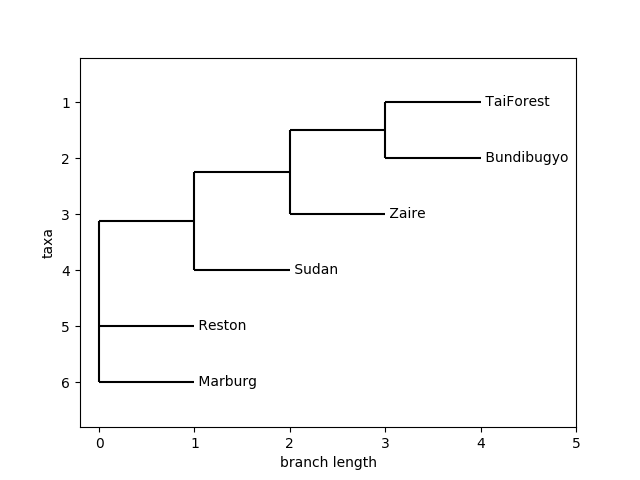
\includegraphics[width=\linewidth]{../Data/Trees/all_and_marburg_NJ.png}
    \caption{all\_and\_marburg\_NJ.png}
  \end{subfigure}
  \begin{subfigure}[b]{0.4\linewidth}
    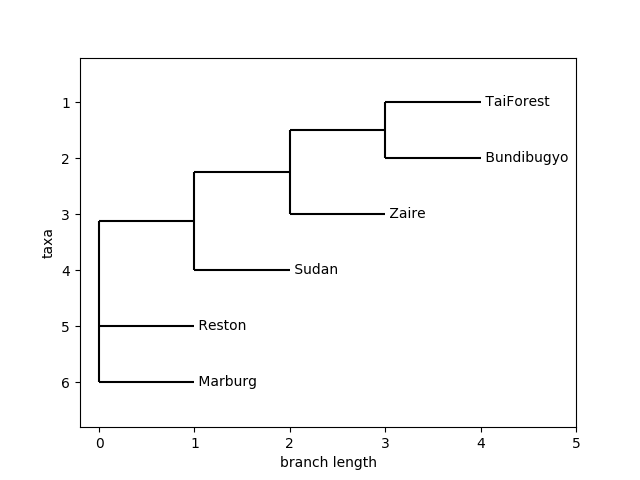
\includegraphics[width=\linewidth]{../Data/Trees/all_and_marburg_NJ.png}
    \caption{all\_and\_marburg\_UPGMA.png}
  \end{subfigure}
\end{figure}
پس  نتیجه می‌گیریم که در ابتدا(یا طبق عبارت صورت سوال نقطه‌ی شروع) ویروسی بوده که به سه گونه‌ی  marburg و Restone و گونه‌ی پدر تمام ویروس‌ها Sudan و Zaire و Taiforest و Bundibugyo جهش پیدا کرده. آن گونه‌ی پدر آخری به Sudan و گونه‌ی پدر گونه‌‌های Zaire و ‌Bundibugyo و TaiForest جهش پیدا کرده. آن گونه‌ی پدر گونه‌‌های  Zaire و ‌Bundibugyo و TaiForest به Zaire و گونه‌ی ‌پدر Bundibugyo و TaiForest جهش پیدا کرده. در نهایت این گونه‌ی پدر آخری به TaiForest و ‌Bundybugyo جهش پیدا کرده.

\section{بخش چهارم}
\subsection{چه زمانی از هم جدا شده‌اند؟}
در این‌جا ما از مدل
\lr{Jukes\_Cantor}
  استفاده کرده‌ایم. علت استفاده از این روش  این است که تنها روشی است که بلد بودیم و البته ساده ‌است و قدرت محاسباتی زیادی به ما می‌دهد(با فرض بازگشت‌پذیر بودن مارکوف‌ها در زمان و غیره). حقیقت این است که چون با روش‌های دیگر آشنا نیستم نمیتوانم بگویم که انتخابی داشته‌ام. اما این روش در کل ساده و منطقی به نظر می‌رسد. مثلا دارد نرخ خطای دی ان ای پلیمراز را مدل می‌کند و منطقی است که این نرخ خطا چندان تغییر نکند. مخصوصا این که ویروس و گونه‌‌هایش در چیزی حدود چند صد سال اخیر به وجود آمده‌اند. در این روش یک ماتریس احتمال به صورت
\begin{figure}[H]
  \centering
  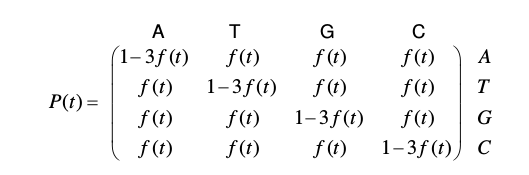
\includegraphics[width=\linewidth]{prob_markov.png}
  \caption{ماتریس احتمال مارکوف}
\end{figure}
داریم که احتمال تبدیل یک نوکلئوتید به دیگر نوکلئوتید‌ها را مدل می‌کند. با این مدل‌سازی و استفاده از تقریب‌هایی که در کلاس استاد مطهری به آن‌ها اشاره شده است می‌توان به این دو نتیجه رسید:

\begin{figure}[H]
  \centering
  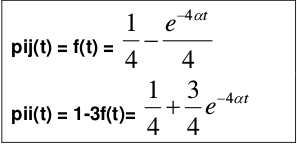
\includegraphics[width=\linewidth]{result.png}
  \caption{ 
نتایج حاصله که در آن‌ها آلفا برابر یک سوم است
  }
  $\alpha = \frac{1}{3}$
\end{figure}

پس با توجه به تعداد تعداد جایگاه‌هایی که دو ژن در آن‌ها به هم شبیه هستند(آن را $b$ بنامید)و تعداد جایگاه‌هایی که در دو ژن متفاوت هستند(آن‌ها را $a$ بنامید). پس احتمال رسیدن دو ویروس به هم را می‌توان در صورت دانستن فاصله‌ی بین آن دو با فرمول:
$$(\frac{1}{4}(1-e^{-\alpha t}))^a\times (\frac{1}{4}(1+3e^{-\alpha t}))^b$$
حساب می‌شود. حال باید $t$‌ای را انتخاب کنیم که احتمال بالا را بیشینه کند. با گرفتن لوگاریتم برای ساده‌تر شدن و انجام محاسبات خواهیم داشت:
\begin{figure}[H]
  \centering
  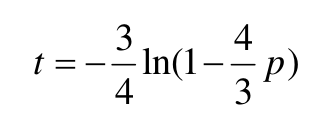
\includegraphics[width=\linewidth]{end_result.png}
  \caption{ 
نتیجه‌ی نهایی
  }
  که در آن 
  $p =\frac{a}{a+b}$
\end{figure}
 البته باید دقت کنیم که در این تصاویر در واقع
 $t = \lambda \times time$
 است که در آن $\lambda$ برابر با نرخ تحول است. پس باید $t$ حاصل در فرمول بالا را بر $\lambda$ که اطلاعات داده شده در صورت پروژه برابر با 
 $1.9\times 10^{-3}$
 در نظر گرفته شده، تقسیم کنیم.
  در این قسمت البته از این 
  \href{http://www.montefiore.ulg.ac.be/~kvansteen/GBIO0009-1/ac20132014/T4/jc.pdf}{منبع}
  استفاده کردیم. حال ما از edit distance به عنوان یک تقریب برای $a$ و از طول یکی از ژنوم‌ها(با توجه به نزدیک بودن طول تمامی ژنوم‌ها) به عنوان یک تقریب برای $a+b$ یا در واقع طول ژنوم استفاده کردیم پس داریم:
  $$p \approx \frac{edit\_distance}{genome\_length}$$
  و سپس یک ماتریس محاسبه کردیم که شامل این فاصله‌های زمانی بود
  \begin{figure}[H]
  \centering
  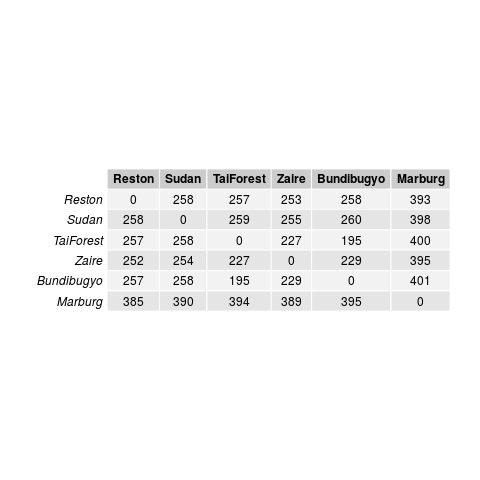
\includegraphics[width=\linewidth]{../Data/Trees/time_matrix.png}
  \caption{ 
فاصله‌‌های زمانی بین گونه‌ها
  }
\end{figure}
  
   و آن را به الگوریتم UPGMA دادیم و طول یال‌ها را برای ما حساب کرد و این نتیجه خروجی شد:
\begin{figure}[H]
\centering
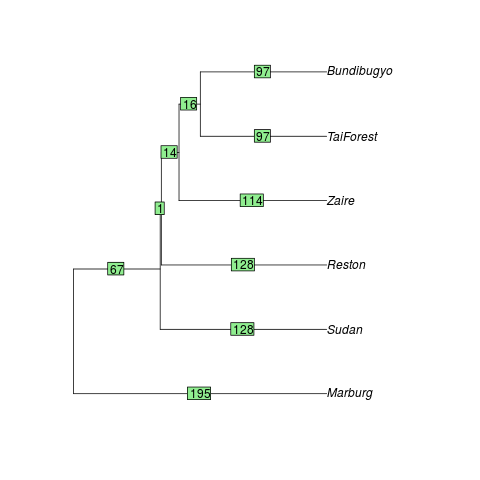
\includegraphics[width=\linewidth]{../Data/Trees/times.png}
\caption{ 
درخت زمانی حاصله
  }
\end{figure}
   که در آن این اعداد نوشته شده در جداول سبز در واقع سال‌های تخمین زده شده هستند، مثلا طبق این جدول marburg 195 سال با پدر این ویروس‌ها فاصله دارد و sudan ۱۲۸ سال با پدر شاخه‌ی ابولا ویروس فاصله دارد و پدر ابولاویروس‌ها ۶۷ سال با پدر مشترکش با ماربرگ ویروس فاصله دارد. پس در کل حدس این است که جد مشترک ابولا ویروس‌ها ۱۲۸ سال قبل میزیسته و پدر مشترک تمام آن‌ها با ماربرگ در ۱۹۵ سال پیش میزیسته(خصوصیت جالب UPGMA که فرض می‌کند تمام برگ‌ها در یک زمان هستند را نیز می‌توانید در تصویر مشاهده کنید).

\end{document}